\documentclass[a4paper]{article}

% ===== Packages =====
\usepackage[T1]{fontenc}        % Font encoding
\usepackage{lmodern}
\usepackage{algorithm}
\usepackage{subcaption}

% Modern font
\usepackage[a4paper,margin=0.8in]{geometry} % Page layout: 1in margin
\usepackage[fleqn]{amsmath}     % Math symbols, left-aligned equations
\setlength{\mathindent}{0pt}    % No indent for fleqn
\usepackage{amssymb}            % Extra math symbols
\usepackage{booktabs}           % Better tables
\usepackage{graphicx}           % Include graphics
\usepackage{setspace}           % Adjust line spacing
\usepackage{titling}            % Customize title format
\usepackage{float}              % [H] for figure placement
\usepackage{color}              % For colored text
\usepackage{booktabs}           % For better tables
\usepackage[colorlinks=true, linkcolor=blue, citecolor=blue, urlcolor=blue]{hyperref}
\usepackage{algorithm}
\usepackage{algorithmic}
\renewcommand{\thealgorithm}{\arabic{algorithm}} % Numerazione autonoma

\newcommand{\todo}[1]{\textcolor{red}{\textbf{TODO:} #1}}

% ===== Line spacing =====
\setstretch{0.9}                % 0.9× spacing; regola a piacere

% ===== Title formatting =====
\pretitle{%
  \begin{center}\bfseries\Large
  }
  \posttitle{%
  \end{center}\vspace{-1em}
}
\preauthor{%
  \begin{center}\small
  }
  \postauthor{%
  \end{center}\vspace{-1em}
}
\predate{}  % no date before
\postdate{} % no date after

% ===== Metadata =====
\title{Report HW3}
\author{%
  \ifdefined\anonymous%
  Anonymous Submission
  \else
  \begin{tabular}{cc}
    Simone De Carli & Damiano Salvaterra \\
    {\small\texttt{simone.decarli@studenti.unitn.it}} &
    {\small\texttt{damiano.salvaterra@studenti.unitn.it}}
  \end{tabular}
  \fi
}
\date{}  % leave date blank

\begin{document}

\maketitle

\section*{Exercise 1}

Given a dataset of approximately $3\cdot 10^4$ entries of the form $(x,y)$, where $x$ is a time value and $y$ is its corresponding value, we are interested in modeling the statistics of the dataset. There is a clear trend in the data.

\subsection*{Part 1: Visualize the trend}

First, we need to visualize the trend in the data. To do this, we scatter plot the data points (\ref{fig:trend-scatter}) and we plot the distribution of the data points (\ref{fig:trend-hist}) that we cannot trust.

\begin{figure}[htbp]
  \centering
  \begin{subfigure}[b]{0.48\textwidth}
    \centering
    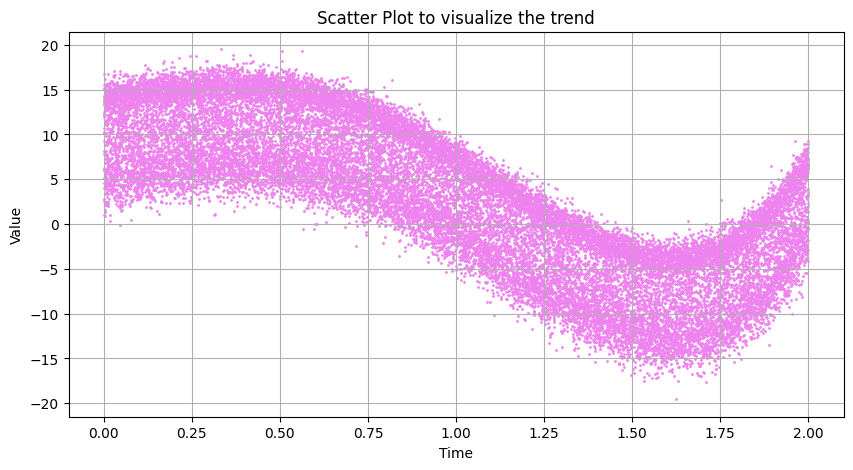
\includegraphics[width=\textwidth]{images/trended_scatter.png}
    \caption{Scatter plot of the dataset.}\label{fig:trend-scatter}
  \end{subfigure}
  \hfill
  \begin{subfigure}[b]{0.48\textwidth}
    \centering
    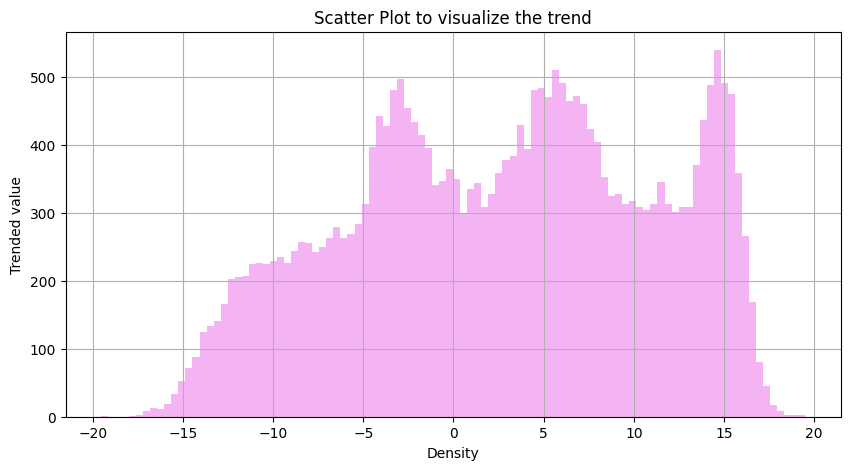
\includegraphics[width=\textwidth]{images/trended_dist.png}
    \caption{Histogram of the dataset.}\label{fig:trend-hist}
  \end{subfigure}
  \caption{Trended dataset.}\label{fig:trend}
\end{figure}

\subsection*{Part 2: Fit a polynomial trend}

We estimate a polynomial trend using the least squares method for degrees from 1 to 8 (\ref{fig:poly-trend}).

\begin{figure}[htbp]
  \centering
  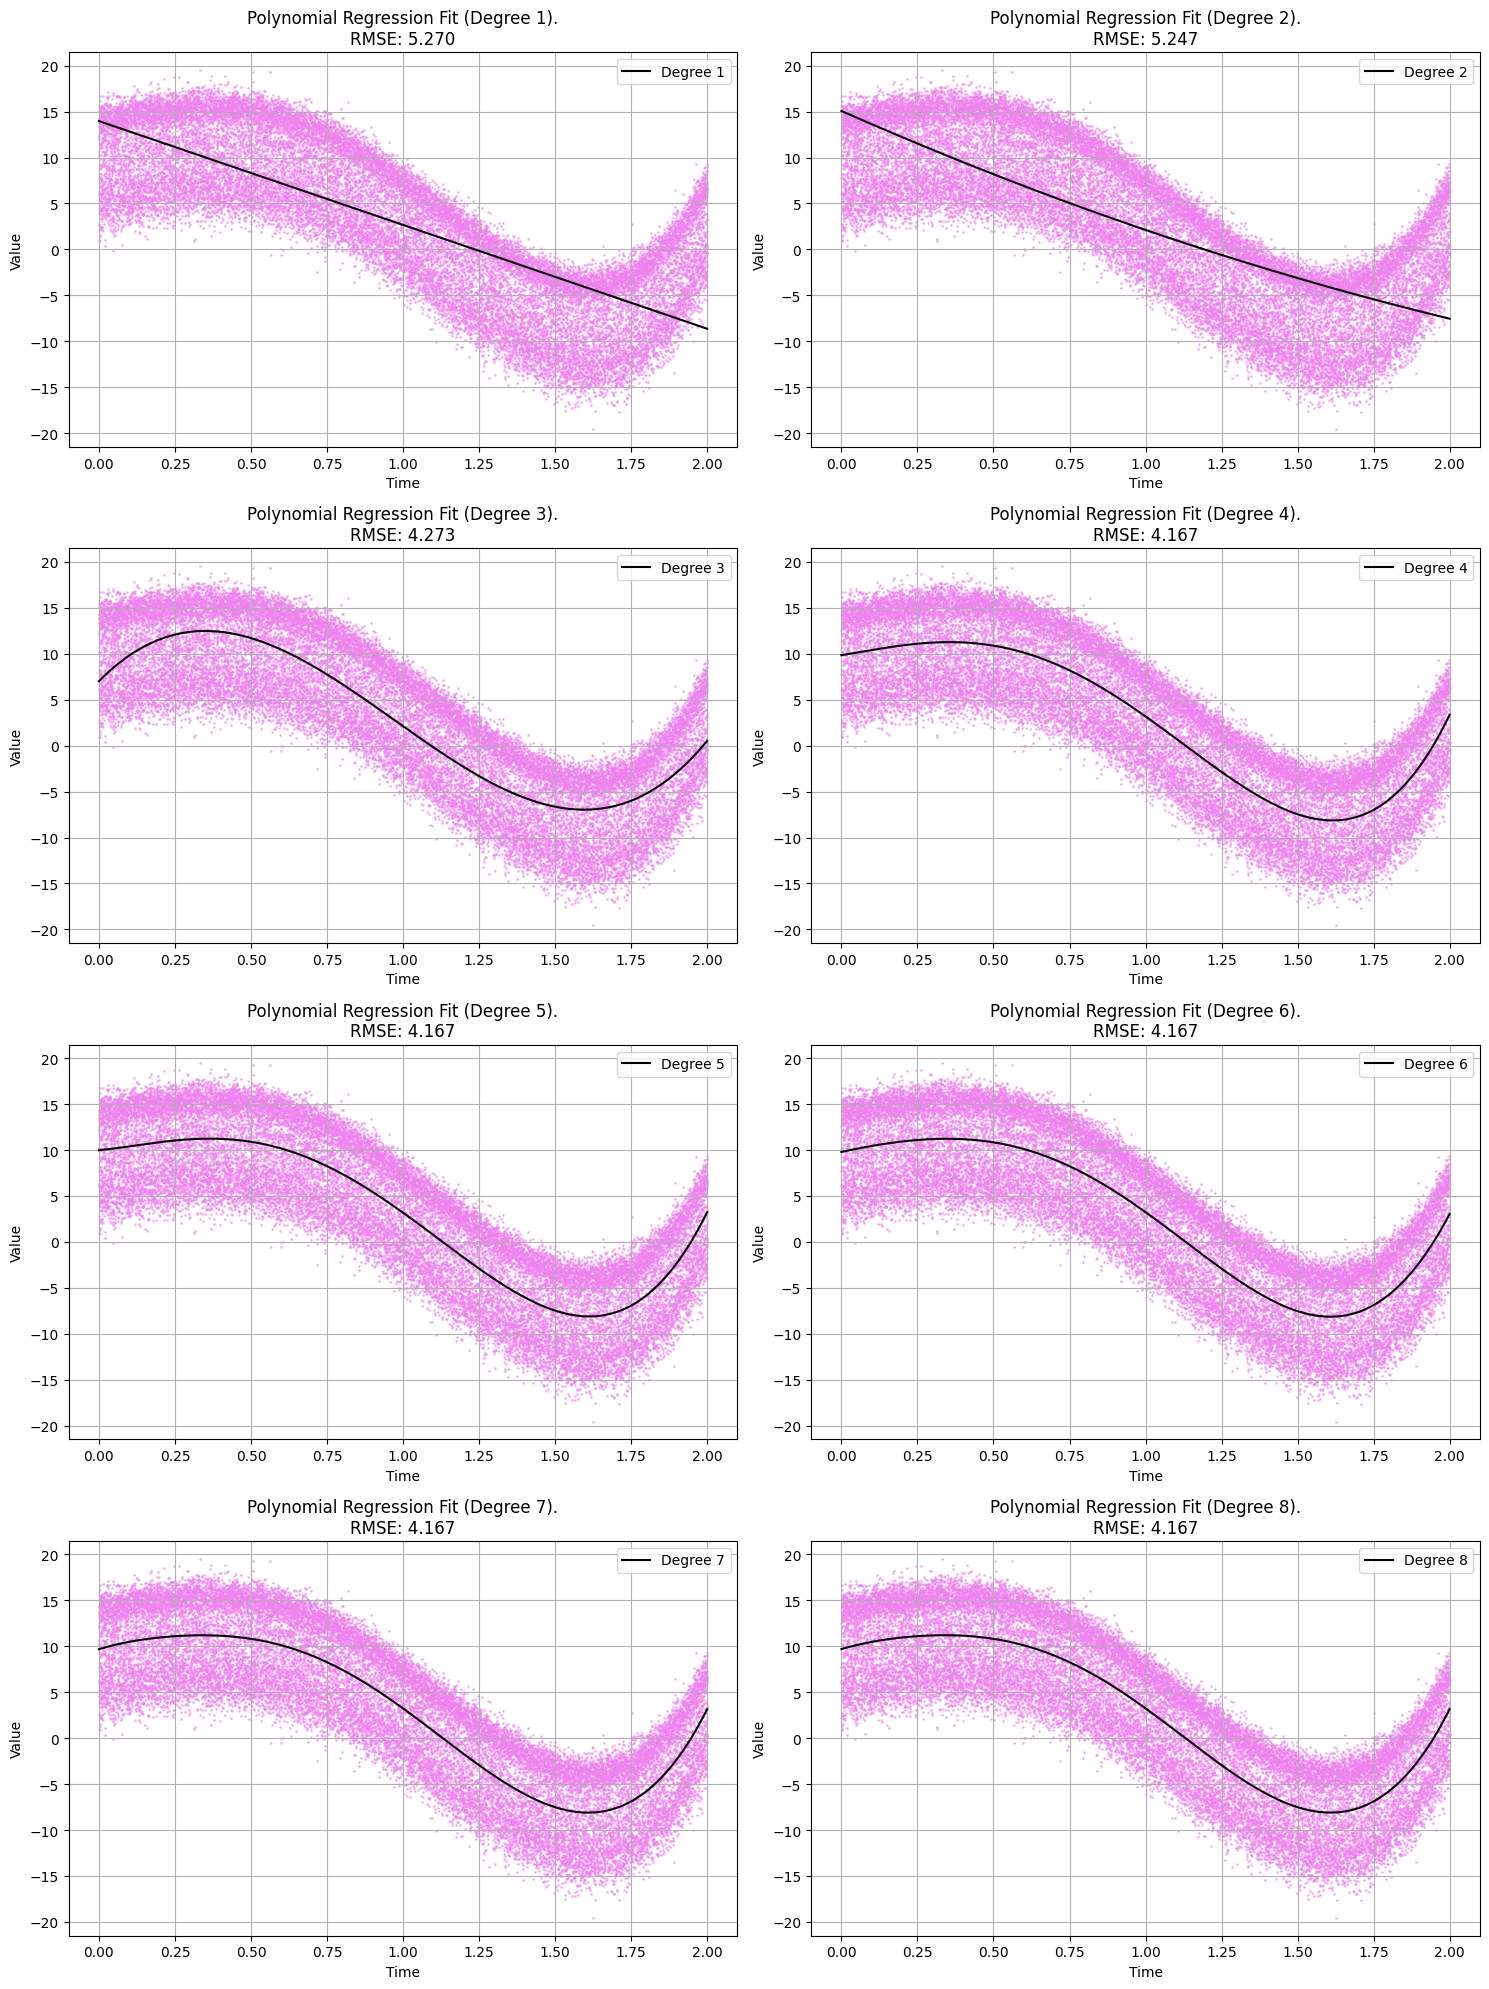
\includegraphics[width=\textwidth]{images/poly_trends.png}\caption{
    Polynomial trends fitted to the dataset.
  }\label{fig:poly-trend}
\end{figure}

\subsection*{Part 3: Find the best degree and remove the trend}

To remove the trend, we need to decide which polynomial degree is the best. Then we can de-trend the data.

\subsubsection*{Find the best degree}



\end{document}
